
\documentclass[preprint,12pt]{elsarticle}

\usepackage[spanish]{babel}
\usepackage{amssymb}
\usepackage{graphicx}
\usepackage{lineno}
\usepackage[utf8]{inputenc}
\usepackage{url}
\usepackage{natbib} 
\usepackage{amsmath} 
\usepackage{amssymb} 

\begin{document}
	
	\begin{frontmatter} 

		\title{\huge Gestores de BD NoSQL}
		
		\author{Estrella Palacios, Katherine Lizbeth      (2016056193))}
		\author{Andia Zeballos,Alonso André           	(2016054945))}
		\author{Porlles Carrillo, Diego Armando	         	(2015050948))}  
		\author{Mamani Mamani, Pedro Luis                 (2010038808))} 
		\address{Escuela Profesional de Ingeniería de Sistemas}
		\address{Universidad Privada de Tacna}
		\address{Tacna, Perú}
		
%% ABSTRACT --------------------------------------------------------------------------------------------------------------------

		\begin{abstract}
		
NoSQL databases have experienced a significant increase in their application in recent times. The great flexibility they offer and the possibilities they offer from the point of view of optimization in their designs according to the problem to be solved make them an attractive variant to consider for developers of information management applications. In this article, we take a look at the evolution of the types of databases until they reach the relational ones, which are analyzed in order to show the aspects associated with them that led to the emergence of the NoSQL. v

		\end{abstract}

%% ----------------------------------------------------------------------------------------------------------------------------------

	\end{frontmatter}

%% RESUMEN ---------------------------------------------------------------------------------------------------------------------

\section{Resumen}

Las bases de datos NoSQL han experimentado un importante incremento en su aplicación en los últimos tiempos. La gran flexibilidad que ofrecen y las posibilidades que brindan desde el punto de vista de la optimización en sus diseños de acuerdo al problema a resolver las convierten en una atractiva variante a tener en cuenta para los desarrolladores de aplicaciones de gestión de información. En el presente artículo se hace un recorrido por la evolución de los tipos de bases de datos hasta llegar a las relacionales, las cuales se analizan con el objetivo de mostrar los aspectos asociados a estas que propiciaron el surgimiento de las NoSQL.

%% ----------------------------------------------------------------------------------------------------------------------------------


%% INTRODUCION ----------------------------------------------------------------------------------------------------------------

\section{Introducción} 

La bases de datos NoSQL ya no son una novedad sino una realidad que encontramos en muchas de las aplicaciones que utilizamos diaramente.
En el pasado habiamos comentado las caracteristicas de este tipo de bases de datos y su evolucion. A direfencia de las bases de datos relacionales, las bases de datos NoSQL no responden a un unico modelo de datos. sino a un conjunto de ellos.
En aras de favorecer la discusión y su comparación, los sistemas gestores de bases de datos NoSQL se clasifican en diferentes familias: los basados en modelos de agregación (que se pueden agrupar en clave-valor, documental o de grandes columnas) y los basados en grafo. Con este post queremos dar inicio a una serie de entradas que sirvan de tutorial a quienes quieran aprender a utilizar bases de datos NoSQL.

\begin{figure}[htb]
	\begin{center}
		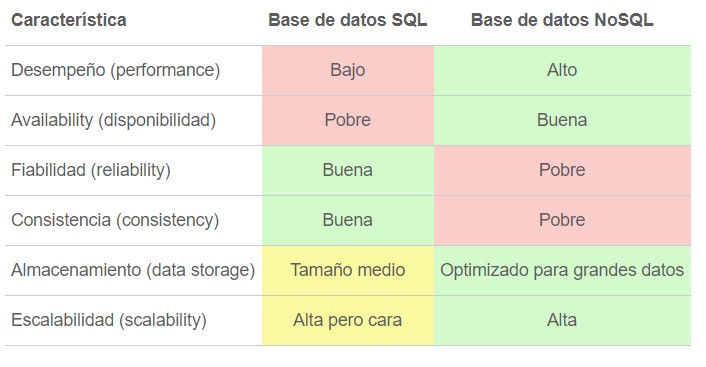
\includegraphics[width=14cm]{./IMAGENES/basededatos_2} 
		\caption{Las bases de datos NoSQL en grafo permiten representar los datos utilizando estructuras de grafos.}
	\end{center}
\end{figure}

%% ----------------------------------------------------------------------------------------------------------------------------------


%% MARCO TEÓRICO ------------------------------------------------------------------------------------------------------------

\section{Marco Teórico}

%% PRIMERA SUBSECCION 

\subsection {\textbf{Definición}}

Una base de datos no relacional (NoSQL) es aquella base de datos que:

\begin{itemize}
	\item No requiere de estructuras de datos fijas como tablas
	\item No garantiza completamente las características ACID
	\item Escala muy bien horizontalmente.
\end{itemize}

Se utilizan en entornos distribuidos que han de estar siempre disponibles y operativos y que gestionan un importante volumen de datos.

%% https://revistadigital.inesem.es/informatica-y-tics/los-gestores-de-bases-de-datos-mas-usados/

\subsubsection{\textbf{Base de datos orientada a Grafos}}

Un grafo estará compuesto por dos elementos: los nodos (vértices) y las relaciones (aristas). Un nodo representa una entidad, en el que almacenaremos piezas de datos o atributos de tipo clave-valor, mientras que las relaciones representan cómo se conectan y se asocian dos nodos.\\

\begin{figure}[htb]
	\begin{center}
		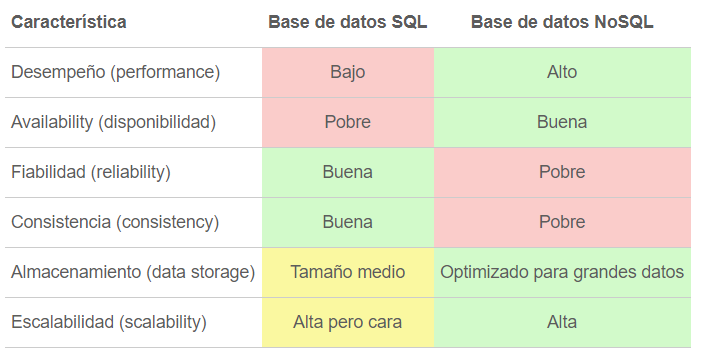
\includegraphics[width=14cm]{./IMAGENES/basededatos_3} 
		\caption{Incluyendo la base de datos en DevOps}
	\end{center}
\end{figure}

Las clasificamos como NoSQL por las siguientes características:
\begin{itemize}
     \item No utilizan un modelo relacional 
     \item Carece de un esquema fijo, podemos tener nodos con diferente número de atributos.  
     \item Mantienen la disponibilidad y acceso de la información
     \item Son buenas en modelos en cluster
\end{itemize}

Sus características principales son:
\begin{itemize}
 \item Son multidimensionales, pueden almacenar atributos de diverso tamaño en los nodos
 \item Las relaciones pueden almacenar atributos
 \item Las relaciones pueden ser sin dirección, unidireccionales y bidireccionales lo que puede convertir la representación a grafos dirigidos, muy útiles en el cálculo de caminos.
 \item Tienen alto rendimiento en la búsqueda de resultados y sobre todo en la búsqueda de caminos.
\end{itemize}
%%Ejemplo de cita
\cite{Gartner} 


\begin{itemize}
	\item x
	\item y
	\item z
\end{itemize}

\subsubsection{\textbf{A2}}

EDITAR\\

\subsubsection{\textbf{A3}}

EDITAR\\


%% SEGUNDA SUBSECCION

\subsection{\textbf{B}}

\subsubsection{\textbf{B1}}

EDITAR\\

%% Ejemplo de inclusión de imagen
\begin{figure}[htb]
	\begin{center}
		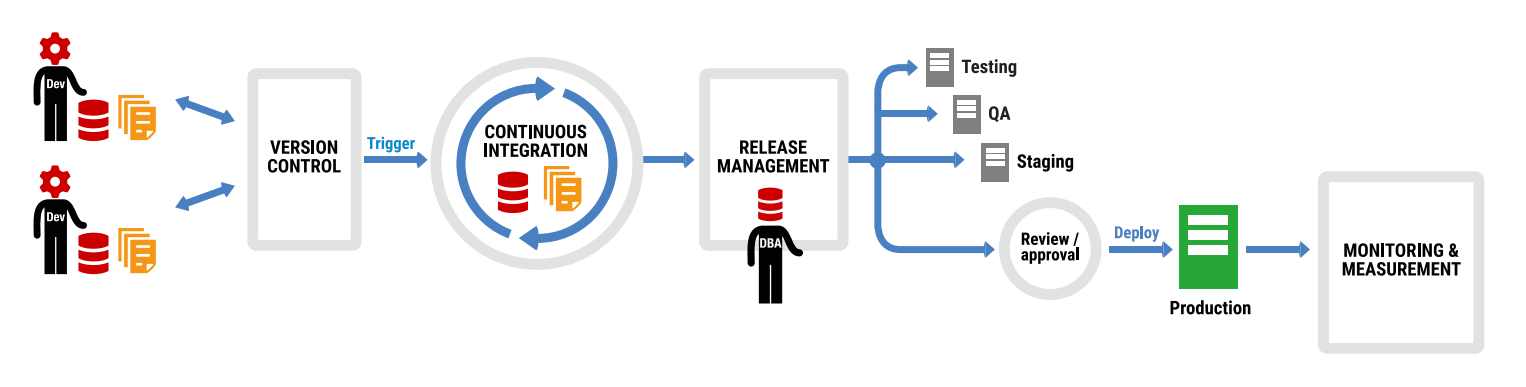
\includegraphics[width=14cm]{./IMAGENES/basededatos_1} 
		\caption{Incluyendo la base de datos en DevOps}
	\end{center}
\end{figure}

\subsubsection{\textbf{B2}}

EDITAR\\

%% TERCERA SUBSECCION
\subsection{\textbf{C}}

\subsubsection{\textbf{C1}}

EDITAR\\

\begin{itemize}

\item x
\item y
\item z

\end{itemize}
\subsubsection{\textbf{C2}}

EDITAR\\


%% ----------------------------------------------------------------------------------------------------------------------------------
 


%% ANÁLISIS ( APLICACIÓN ) ---------------------------------------------------------------------------------------------------

\section{Análisis}

\subsection{\textbf{Base de datos orientada a Grafos. ¿Qué son y para qué se usan?}}
¿Qué son las bases de datos orientadas a Grafos? Lo más probable es que hayas empezado a escuchar algo sobre este tipo de bases de datos, que si son capaces de detectar el fraude.\\

¿En qué contextos las podemos usar?

Las BDOG están pensadas para aquellos ámbitos en donde es importante mantener un modelo extenso y amplio de la relación de la información a la vez que un esquema flexible de los datos. Podemos ver un ejemplo claro en las redes sociales, como Twitter o Facebook, donde tenemos el número de conexiones como las relaciones con nosotros y las personas como nodos del grafo.

“Las bases de datos de grafos no son nuevas, pero solventan un problema subyacente de las documentales”



\subsection{\textbf{Análisis 2}}
EDITAR\\

\subsection{\textbf{Análisis 3}}
EDITAR\\

\subsection{\textbf{Análisis 4}}
EDITAR\\

%% ----------------------------------------------------------------------------------------------------------------------------------


%% CONCLUSIONES ---------------------------------------------------------------------------------------------------------------

\section{Conclusiones}

\begin{itemize}

\item Como hemos visto a lo largo del artículo, las BDOG nos ofrecen una gran versatilidad frente a otros modelos de tipos NoSQL y las recomendamos utilizar en los casos en los que se haga un principal hincapié en las relaciones de relación entre las entidades junto con un modelo de la información datos, flexible. Además, los algoritmos de búsqueda, descubrimiento de caminos cortos, exploración en anchura y profundidad que incluyen estas base de datos son temas que resultan muy interesantes seguir aprendiendo sobre ello.\\

\item Conclusion 2 : \\ 

\item Conclusion 3 : \\ 

\item Conclusion 4 : \\ 
\end{itemize}

%% ----------------------------------------------------------------------------------------------------------------------------------

%%  REFERENCIAS BIBLIOGRÁFICAS ------------------------------------------------------------------------------------------
	
	\newpage
	
	\bibliographystyle{apalike} 	%ESTILO
	\bibliography{BIBLIOGRAFIA}	 
	
	
\end{document}
